\begin{minipage}{0.75\linewidth}
\begin{figure}[h]
    \centering
    \begin{adjustbox}{max width=1.0\linewidth, keepaspectratio}
        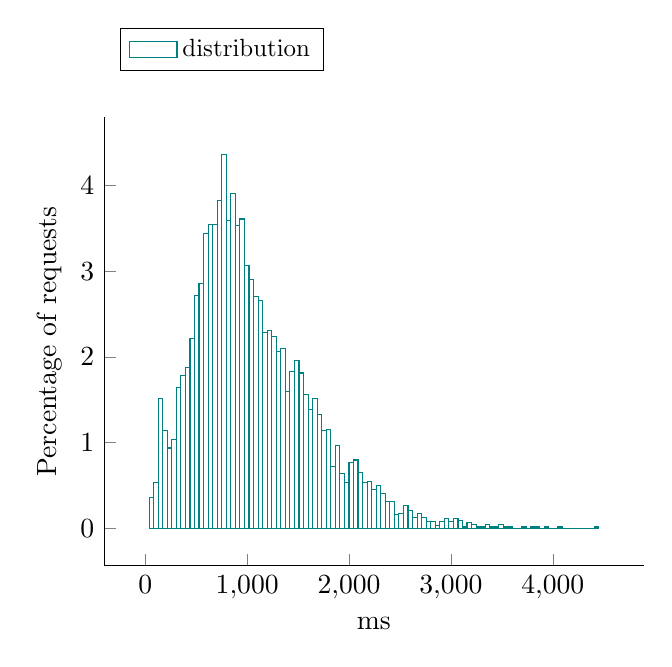
\begin{tikzpicture}
            \begin{axis}[ylabel = Percentage of requests, 
xlabel = ms, 
legend style = {nodes={scale=0.9, transform shape}, at={(0.03,1.2)}, anchor=north west, draw=black, fill=white, align=left, legend columns=3},
area style, mark size = 0pt,
 cycle list name = exotic,
  axis lines* = left]
		\addplot +[ybar interval] coordinates {
			 (37, 0.359375)
			 (81.59, 0.53125)
			 (126.18, 1.51562)
			 (170.77, 1.14062)
			 (215.36, 0.9375)
			 (259.95, 1.03125)
			 (304.54, 1.64062)
			 (349.13, 1.78125)
			 (393.72, 1.875)
			 (438.31, 2.21875)
			 (482.9, 2.71875)
			 (527.49, 2.85938)
			 (572.08, 3.4375)
			 (616.67, 3.54688)
			 (661.26, 3.54688)
			 (705.85, 3.82813)
			 (750.44, 4.35938)
			 (795.03, 3.59375)
			 (839.62, 3.90625)
			 (884.21, 3.53125)
			 (928.8, 3.60938)
			 (973.39, 3.0625)
			 (1017.98, 2.90625)
			 (1062.57, 2.70312)
			 (1107.16, 2.65625)
			 (1151.75, 2.28125)
			 (1196.34, 2.3125)
			 (1240.93, 2.23438)
			 (1285.52, 2.0625)
			 (1330.11, 2.09375)
			 (1374.7, 1.59375)
			 (1419.29, 1.82812)
			 (1463.88, 1.95312)
			 (1508.47, 1.8125)
			 (1553.06, 1.5625)
			 (1597.65, 1.39062)
			 (1642.24, 1.51562)
			 (1686.83, 1.32812)
			 (1731.42, 1.14062)
			 (1776.01, 1.15625)
			 (1820.6, 0.71875)
			 (1865.19, 0.96875)
			 (1909.78, 0.640625)
			 (1954.37, 0.53125)
			 (1998.96, 0.765625)
			 (2043.55, 0.796875)
			 (2088.14, 0.65625)
			 (2132.73, 0.53125)
			 (2177.32, 0.546875)
			 (2221.91, 0.453125)
			 (2266.5, 0.5)
			 (2311.09, 0.40625)
			 (2355.68, 0.3125)
			 (2400.27, 0.3125)
			 (2444.86, 0.15625)
			 (2489.45, 0.171875)
			 (2534.04, 0.265625)
			 (2578.63, 0.203125)
			 (2623.22, 0.125)
			 (2667.81, 0.171875)
			 (2712.4, 0.125)
			 (2756.99, 0.078125)
			 (2801.58, 0.078125)
			 (2846.17, 0.03125)
			 (2890.76, 0.078125)
			 (2935.35, 0.109375)
			 (2979.94, 0.078125)
			 (3024.53, 0.109375)
			 (3069.12, 0.09375)
			 (3113.71, 0.015625)
			 (3158.3, 0.0625)
			 (3202.89, 0.046875)
			 (3247.48, 0.015625)
			 (3292.07, 0.015625)
			 (3336.66, 0.046875)
			 (3381.25, 0.015625)
			 (3425.84, 0.015625)
			 (3470.43, 0.046875)
			 (3515.02, 0.015625)
			 (3559.61, 0.015625)
			 (3604.2, 0)
			 (3648.79, 0)
			 (3693.38, 0.015625)
			 (3737.97, 0)
			 (3782.56, 0.015625)
			 (3827.15, 0.015625)
			 (3871.74, 0)
			 (3916.33, 0.015625)
			 (3960.92, 0)
			 (4005.51, 0)
			 (4050.1, 0.015625)
			 (4094.69, 0)
			 (4139.28, 0)
			 (4183.87, 0)
			 (4228.46, 0)
			 (4273.05, 0)
			 (4317.64, 0)
			 (4362.23, 0)
			 (4406.82, 0.015625)
			 (4451.41, 0)
		};
\addlegendentry{distribution};
           \end{axis}
      \end{tikzpicture}
  \end{adjustbox}
  \caption{Response time distribution - req = ReadTimeline-3}
\end{figure}
\end{minipage}\hfill\begin{minipage}{0.18\linewidth}
\begin{table}[h]
\begin{tabular}{|cc|}
\hline
\textbf{} & \textbf{ms}\\ \hline
 \Xhline{0.005\arrayrulewidth}
min & 37\\
 \Xhline{0.005\arrayrulewidth}
max & 4496\\
 \Xhline{0.005\arrayrulewidth}
mean & 1063\\
 \Xhline{0.005\arrayrulewidth}
std & 580\\
\hline
\hline
 \Xhline{0.005\arrayrulewidth}
25th & 655\\
 \Xhline{0.005\arrayrulewidth}
50th & 949\\
 \Xhline{0.005\arrayrulewidth}
75th & 1398\\
 \Xhline{0.005\arrayrulewidth}
80th & 1521\\
 \Xhline{0.005\arrayrulewidth}
85th & 1658\\
 \Xhline{0.005\arrayrulewidth}
90th & 1846\\
 \Xhline{0.005\arrayrulewidth}
95th & 2168\\
 \Xhline{0.005\arrayrulewidth}
99th & 2802\\
\hline
\end{tabular}
\caption{Response time}
\end{table}
\end{minipage}\hfill